The following subsections present the results only. The results have been discussed in a later section.

\subsection{Cantera}

The results for the rich zone are presented below generated using the \textit{report} method in cantera:

\clearpage

\begin{minted}[frame=lines,fontsize=\footnotesize,linenos, baselinestretch=1.0]{bash}
Phi=1.24: Outlet temperature = 2217.4 K

  gas:

       temperature   2217.4 K
          pressure   1.2e+06 Pa
           density   1.5189 kg/m^3
  mean mol. weight   23.336 kg/kmol
   phase of matter   gas

                          1 kg             1 kmol     
                     ---------------   ---------------
          enthalpy             41090        9.5886e+05  J
   internal energy       -7.4898e+05       -1.7478e+07  J
           entropy             10359        2.4173e+05  J/K
    Gibbs function       -2.2929e+07       -5.3507e+08  J
 heat capacity c_p            1758.2             41028  J/K
 heat capacity c_v            1401.9             32714  J/K

                      mass frac. Y      mole frac. X     chem. pot. / RT
                     ---------------   ---------------   ---------------
                N2           0.76963           0.73853            -24.18
                 H        1.8748e-09        4.9999e-08           -14.749
                O2           0.12591           0.10578           -27.926
                OH        0.00012524        0.00019796           -28.716
                 O        1.9361e-06         3.253e-06            -13.96
                H2        1.6296e-07         2.173e-06           -29.498
               H2O           0.10401            0.1552           -43.471
               HO2         1.016e-06        8.2747e-07           -42.678
              H2O2        1.1488e-07        9.0793e-08           -57.432
                NO        0.00031302        0.00028043           -27.924
\end{minted}

The results after the lean region, i.e. the combustor outlet are presented below:

\begin{minted}[frame=lines,fontsize=\footnotesize,linenos, baselinestretch=1.0]{shell}
Phi=0.42: Outlet temperature = 1675.5 K

  gas:

       temperature   1675.5 K
          pressure   1.2e+06 Pa
           density   2.3156 kg/m^3
  mean mol. weight   26.882 kg/kmol
   phase of matter   gas

                          1 kg             1 kmol     
                     ---------------   ---------------
          enthalpy        3.4244e+05        9.2055e+06  J
   internal energy       -1.7579e+05       -4.7255e+06  J
           entropy            8732.5        2.3475e+05  J/K
    Gibbs function       -1.4289e+07       -3.8411e+08  J
 heat capacity c_p            1399.2             37614  J/K
 heat capacity c_v            1089.9             29299  J/K

                      mass frac. Y      mole frac. X     chem. pot. / RT
                     ---------------   ---------------   ---------------
                N2           0.77429           0.64498           -25.251
                 H        2.0651e-05        0.00047808           -9.9996
                O2        3.0781e-06        2.2448e-06           -39.673
                OH        0.00022282        0.00030573           -29.836
                 O        9.0035e-07        1.3132e-06           -19.836
                H2         0.0060517           0.07005           -19.999
               H2O           0.21935           0.28413           -39.836
               HO2        5.1905e-09        3.6697e-09           -49.673
              H2O2          7.66e-09        5.2552e-09           -59.672
                NO         5.847e-05        4.5472e-05           -32.309
                
NOx at outlet: 58.47 ppm
\end{minted}

\subsection{Simulation}

Analyzing the velocity field is essential, as it directly influences flame length, fuel-air mixing quality, and residence time within the combustion chamber—all of which affect combustion stability and \ce{NOx} formation. The profiles show the effectiveness of the swirlers in mixing the fuel with the air. This can be further seen when the species mass fractions are presented.

\begin{figure}[H]
\centering
\begin{subfigure}[b]{0.49\textwidth}   
    \centering 
    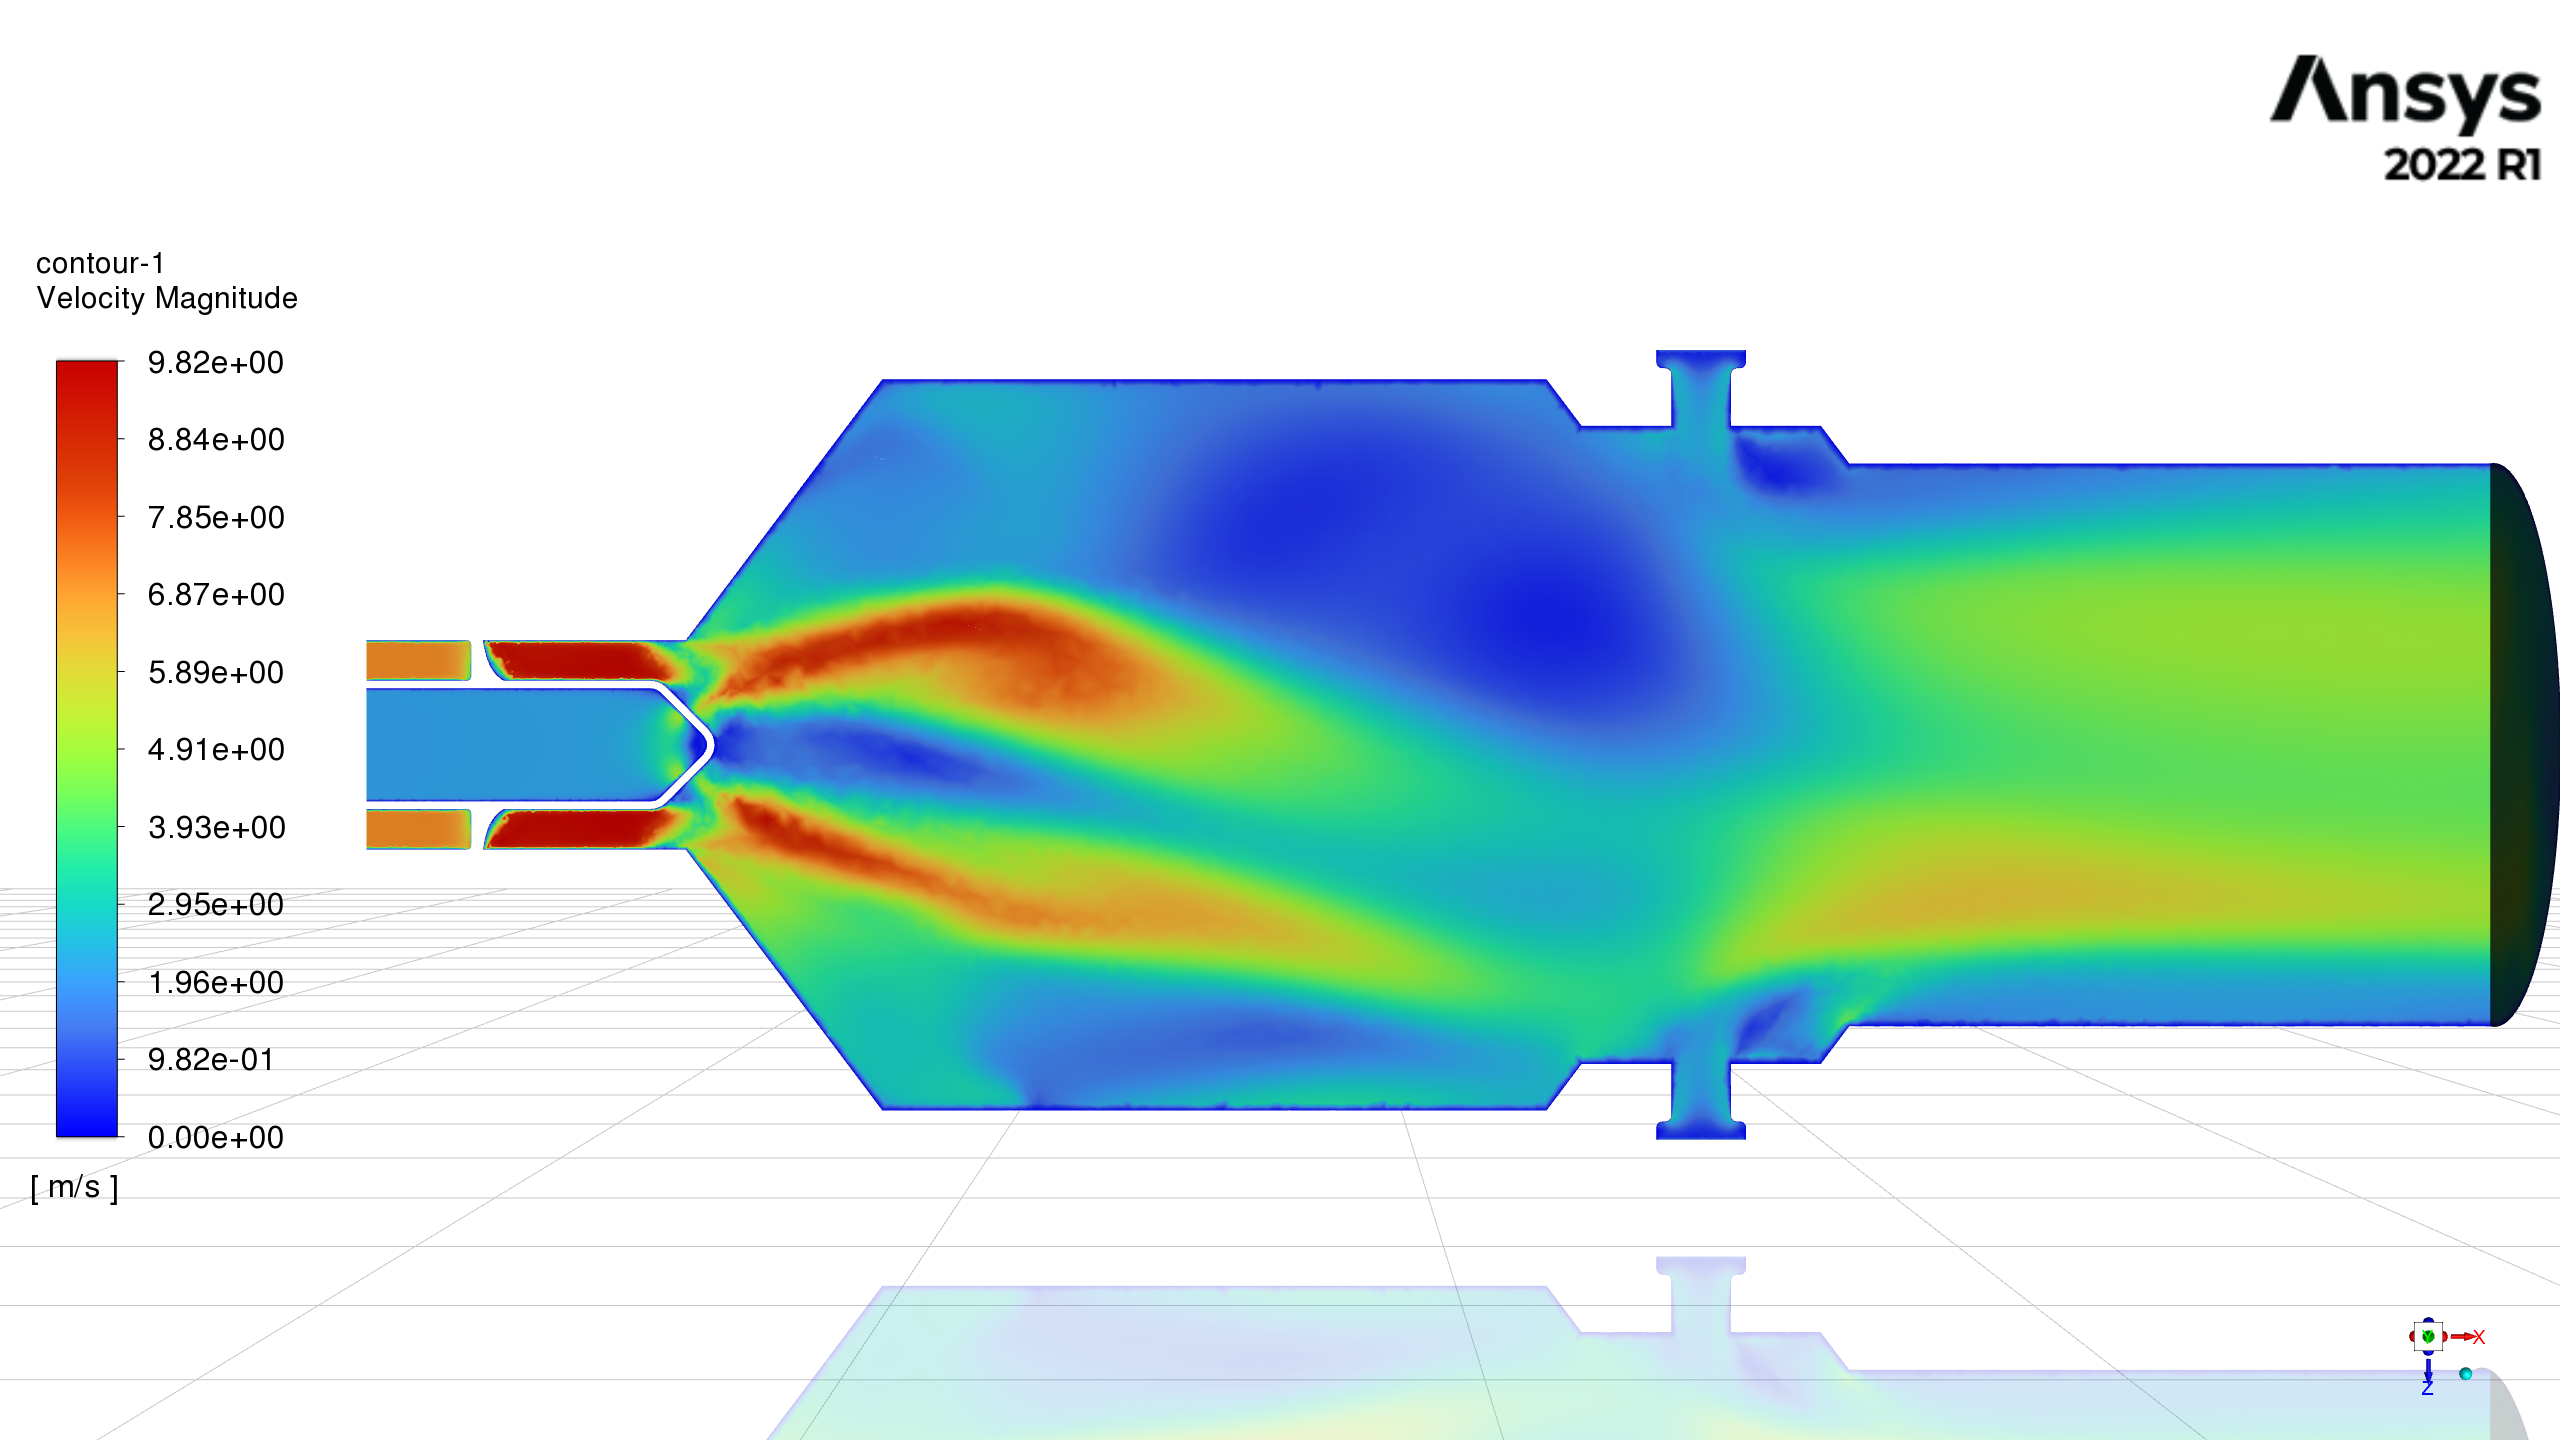
\includegraphics[width=\textwidth]{figs/velocity.png}
\end{subfigure}
\hfill
\begin{subfigure}[b]{0.49\textwidth}   
    \centering 
    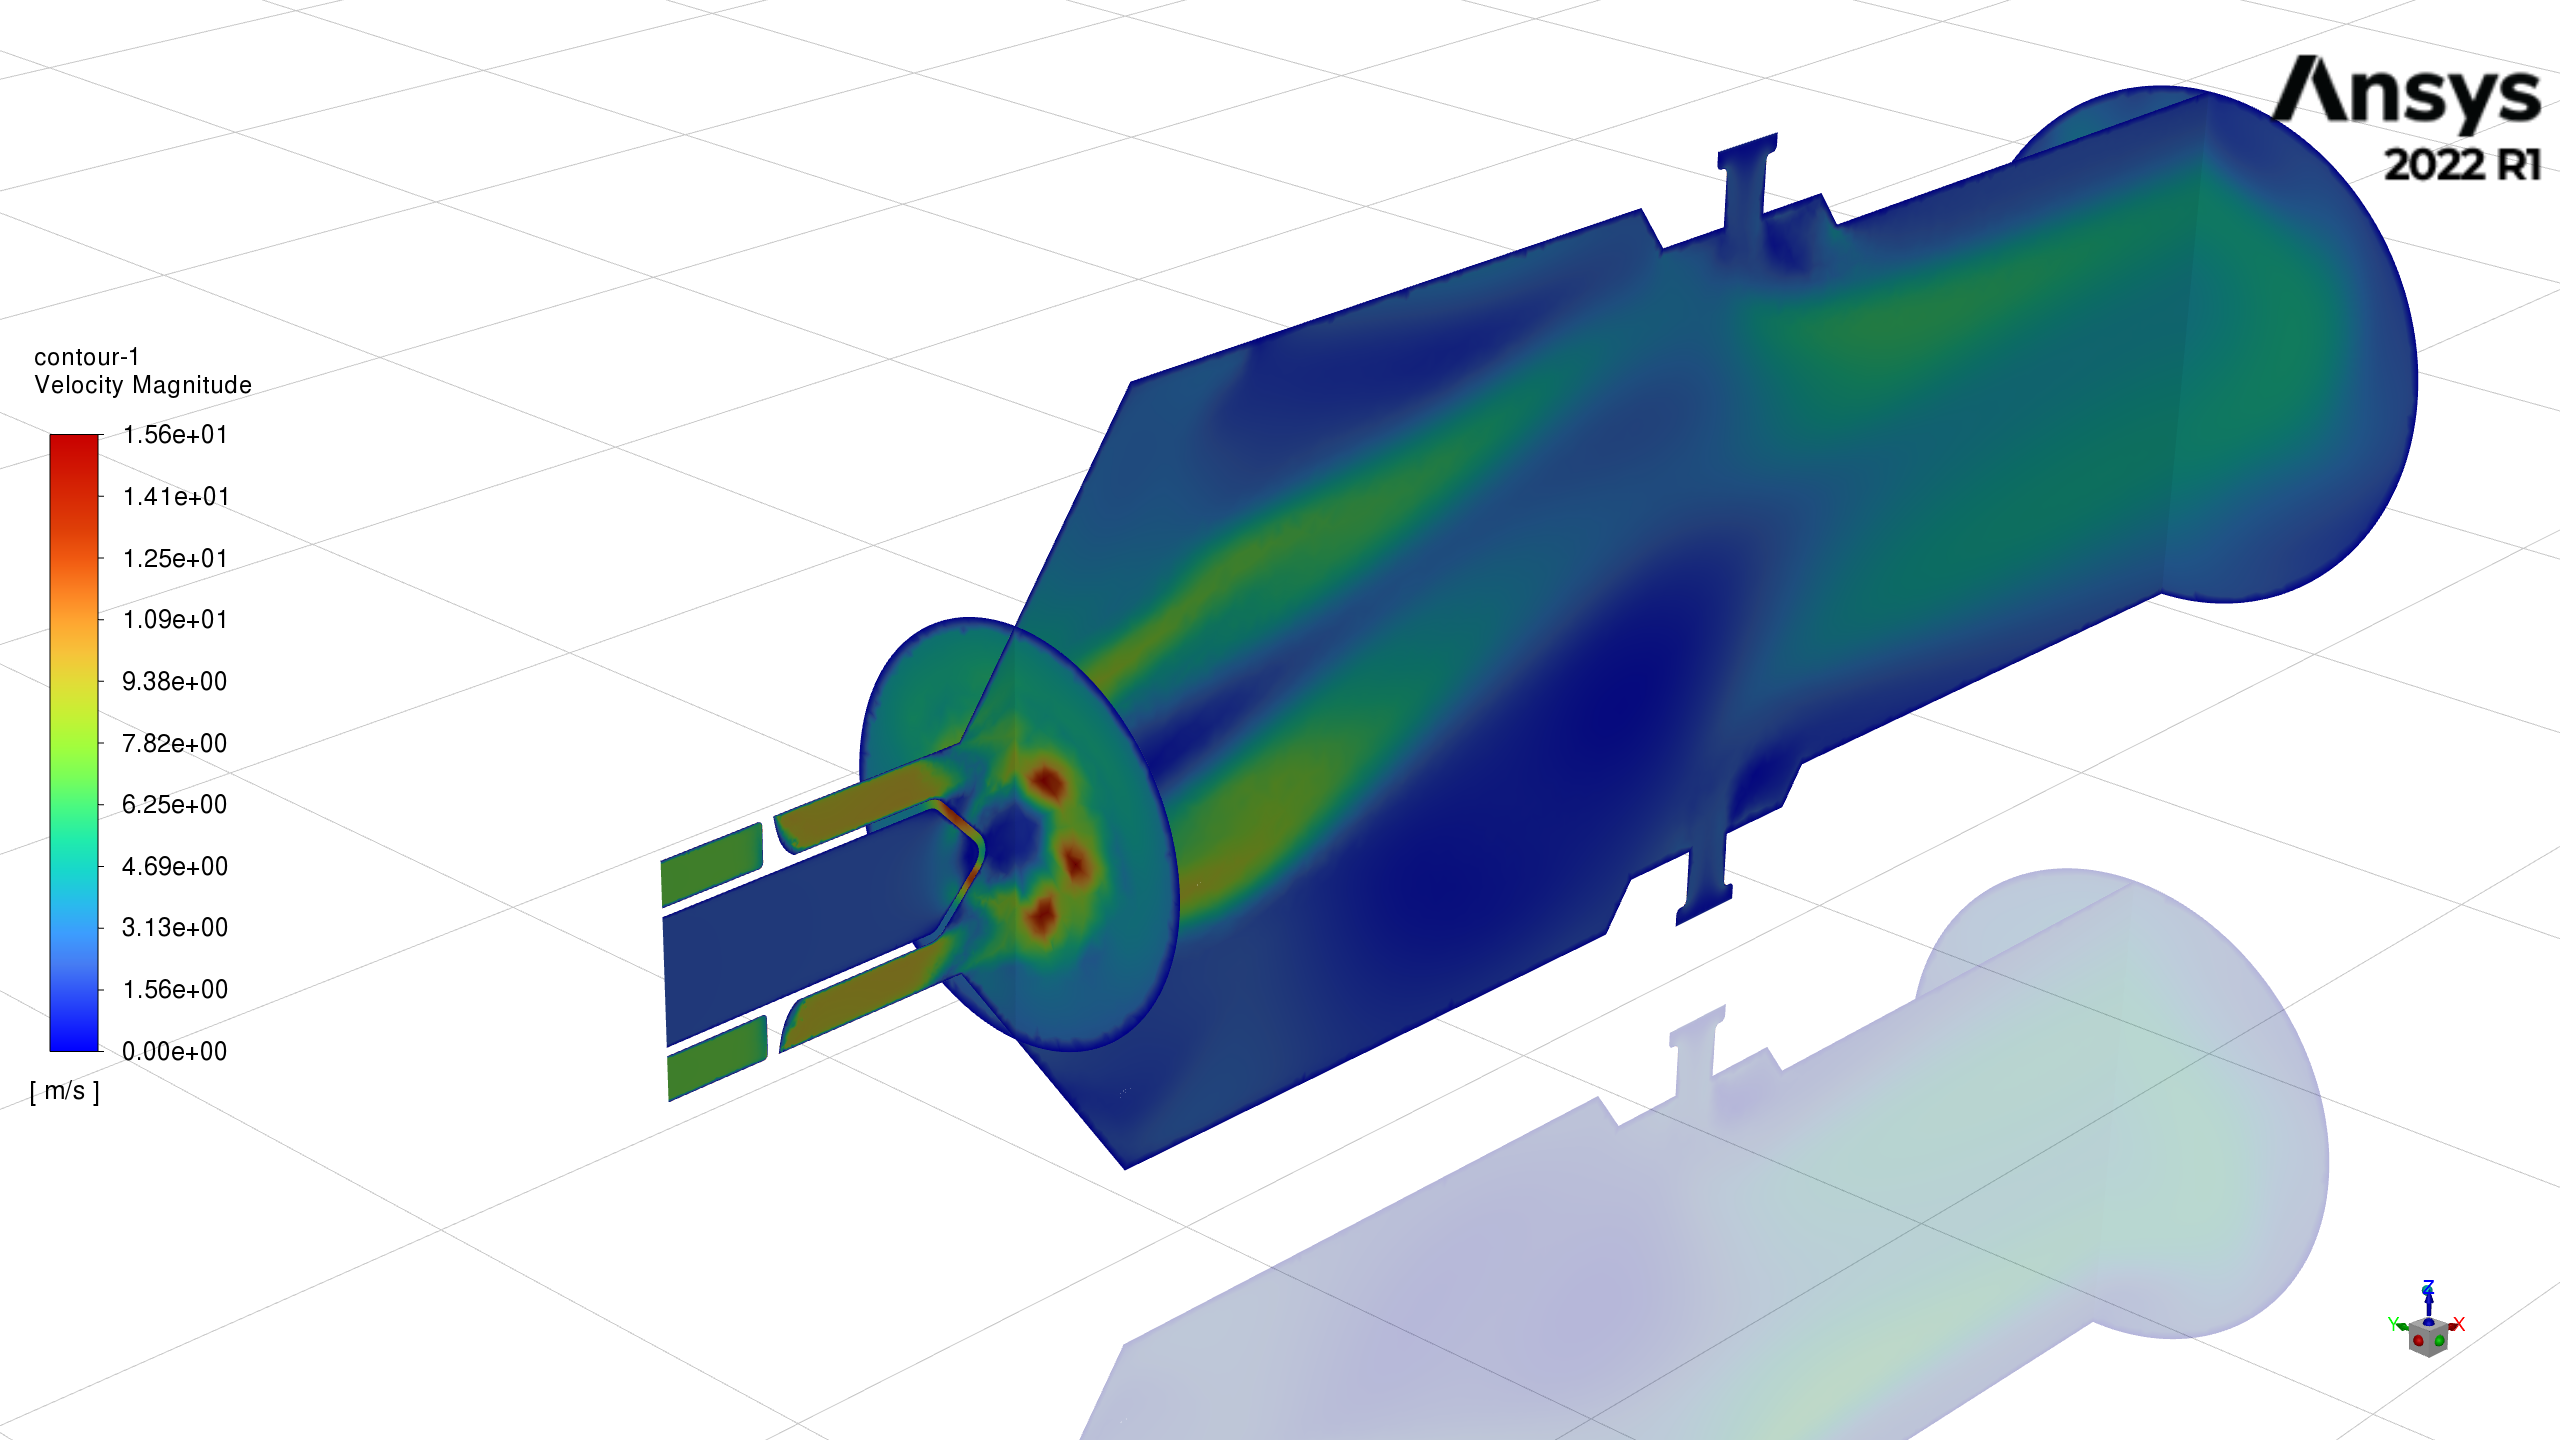
\includegraphics[width=\textwidth]{figs/velocity_front.png}
\end{subfigure}
\caption{Velocity profile for the combustor.} \label{fig:velocity_field}
\end{figure}


One of the most important factors that determines the success of the injector is the temperature of the mixture in the combustion system, as it is the only factor responsible for the production of \ce{NOx}. We know that \ce{NOx} is being produced when the flame is above 1850 K. The temperatures within combustor reach around 2300 K. This indicates that \ce{NOx} are being produced. However, as the cooling air is added, the temperature drops, neutralizing the radicals responsible for emissions. One can look at the mass fraction of \ce{NO} to calculate the the amount of emissions being produced. This will be seen when the species are discussed.

\begin{figure}[H]
\centering
\begin{subfigure}[b]{0.49\textwidth}   
    \centering 
    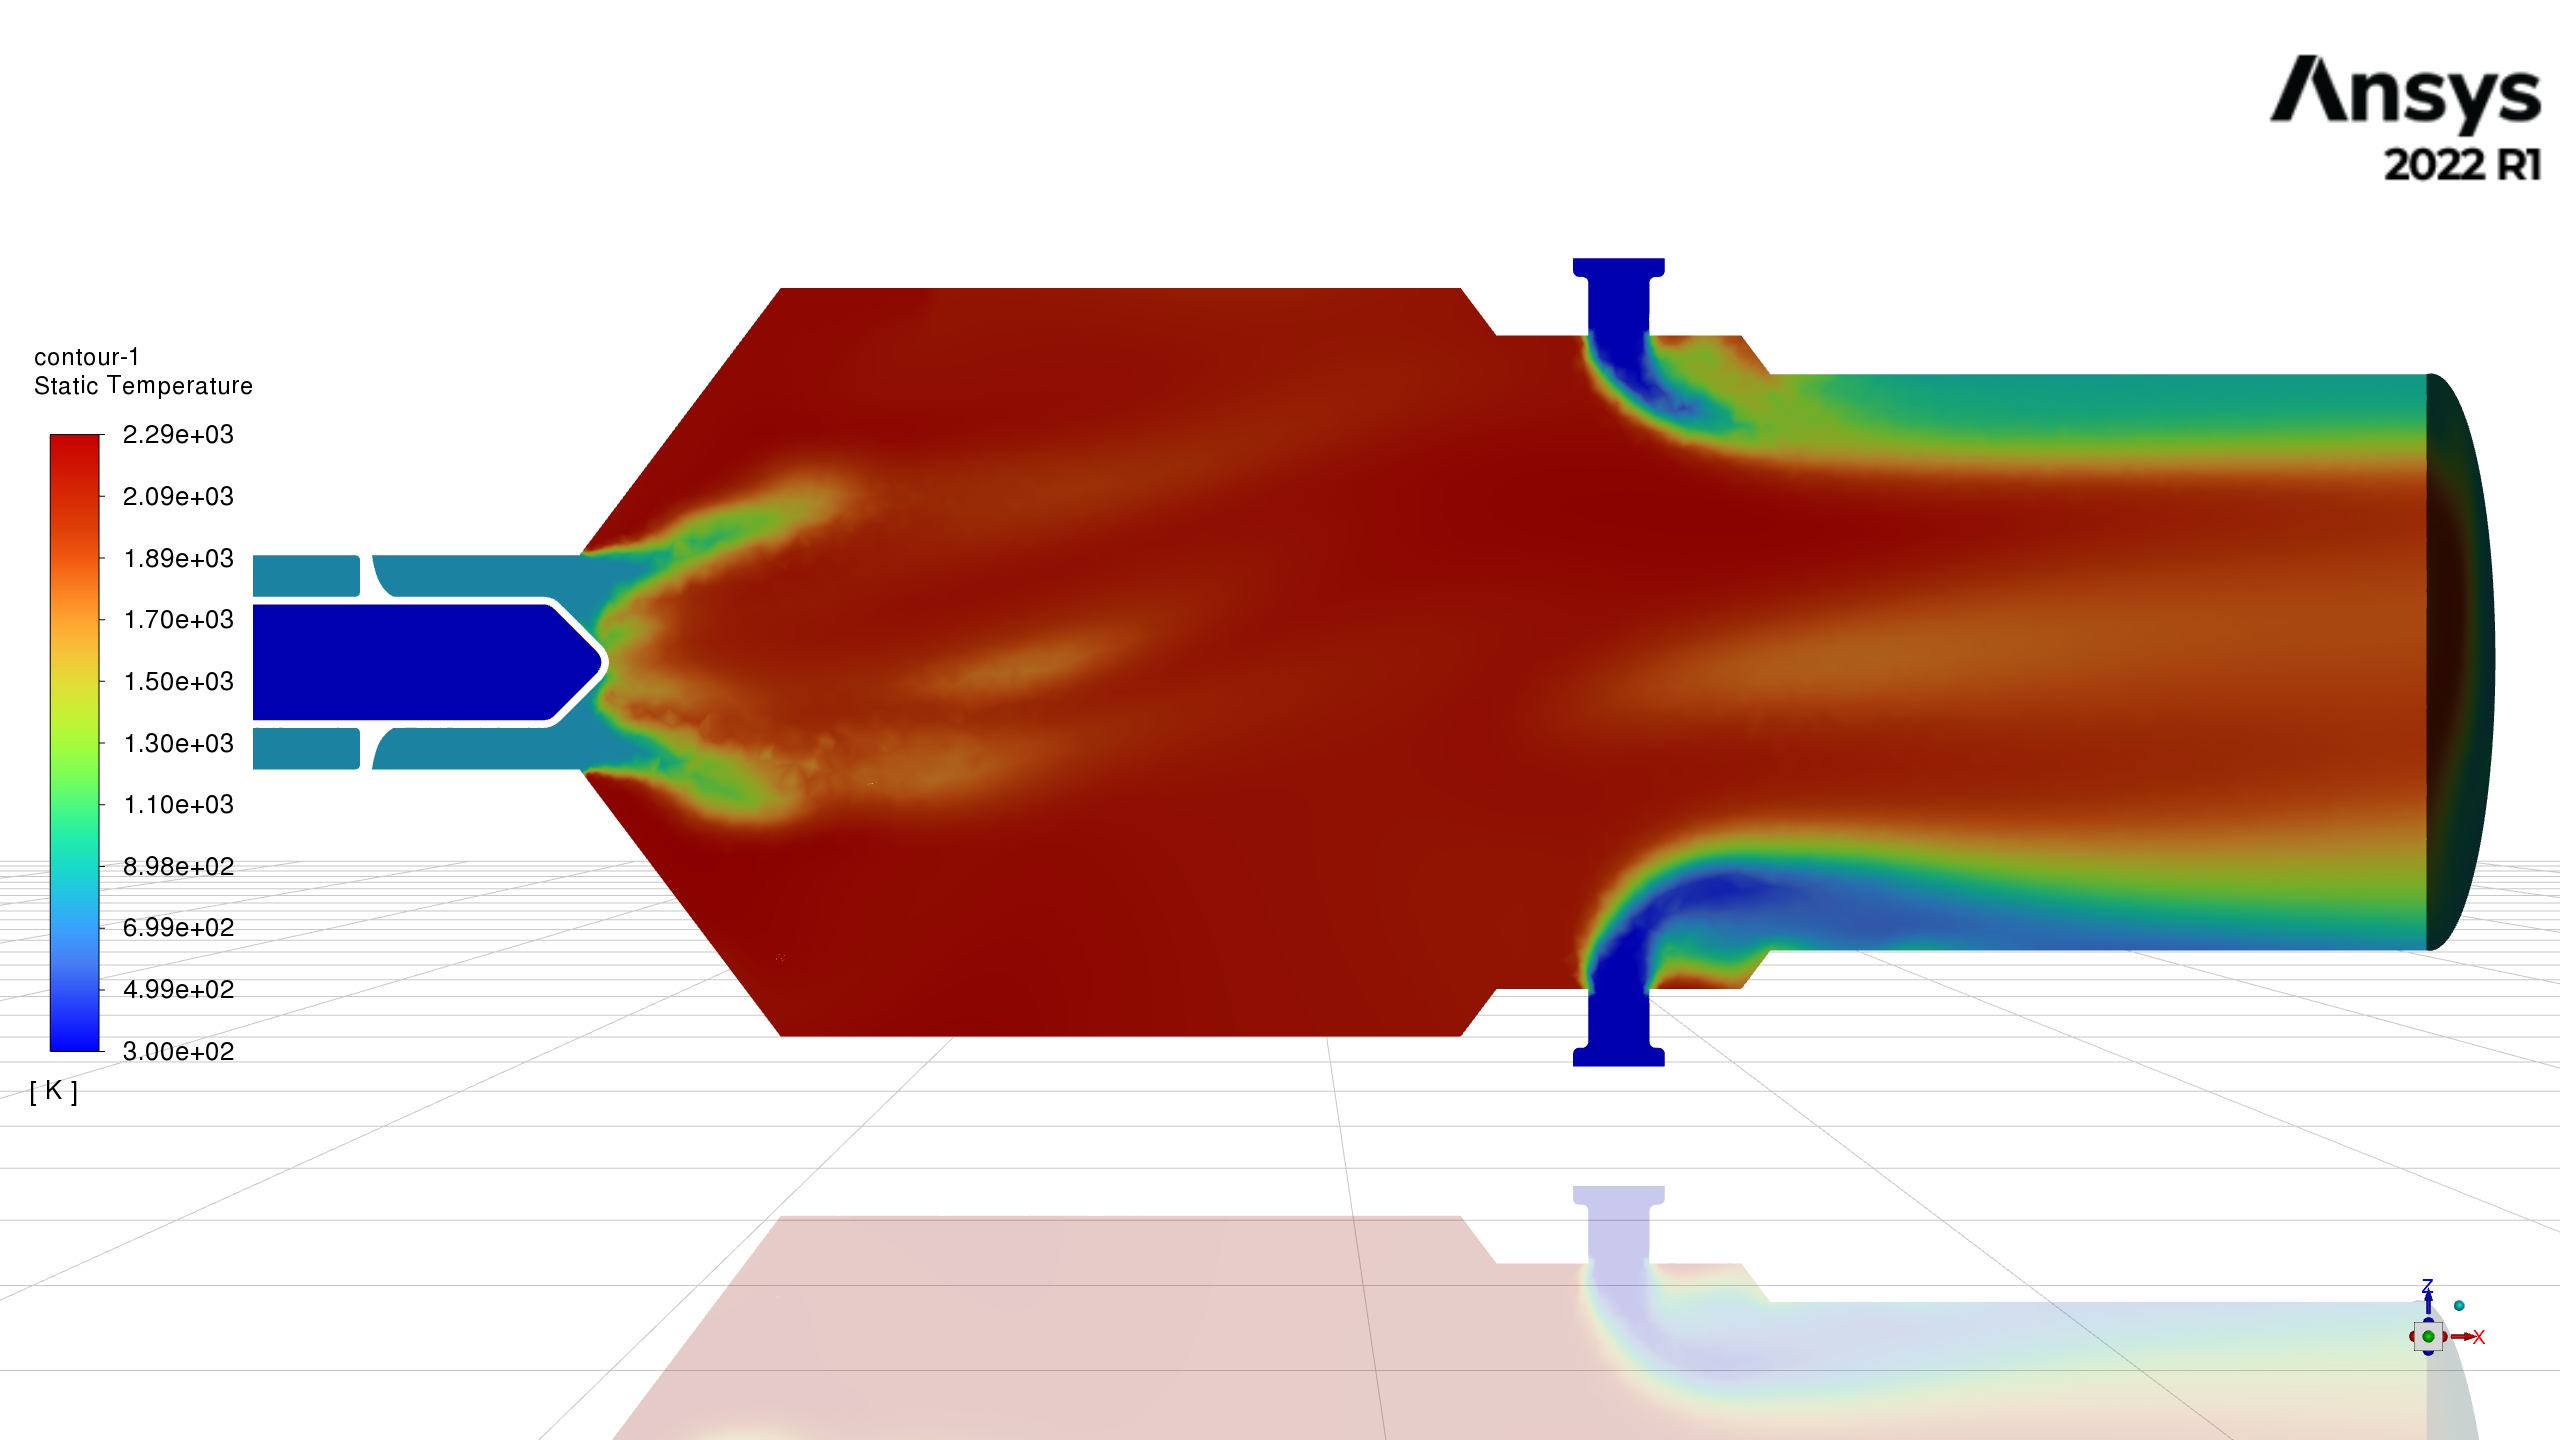
\includegraphics[width=\textwidth]{figs/temperature.png}
\end{subfigure}
\hfill
\begin{subfigure}[b]{0.49\textwidth}   
    \centering 
    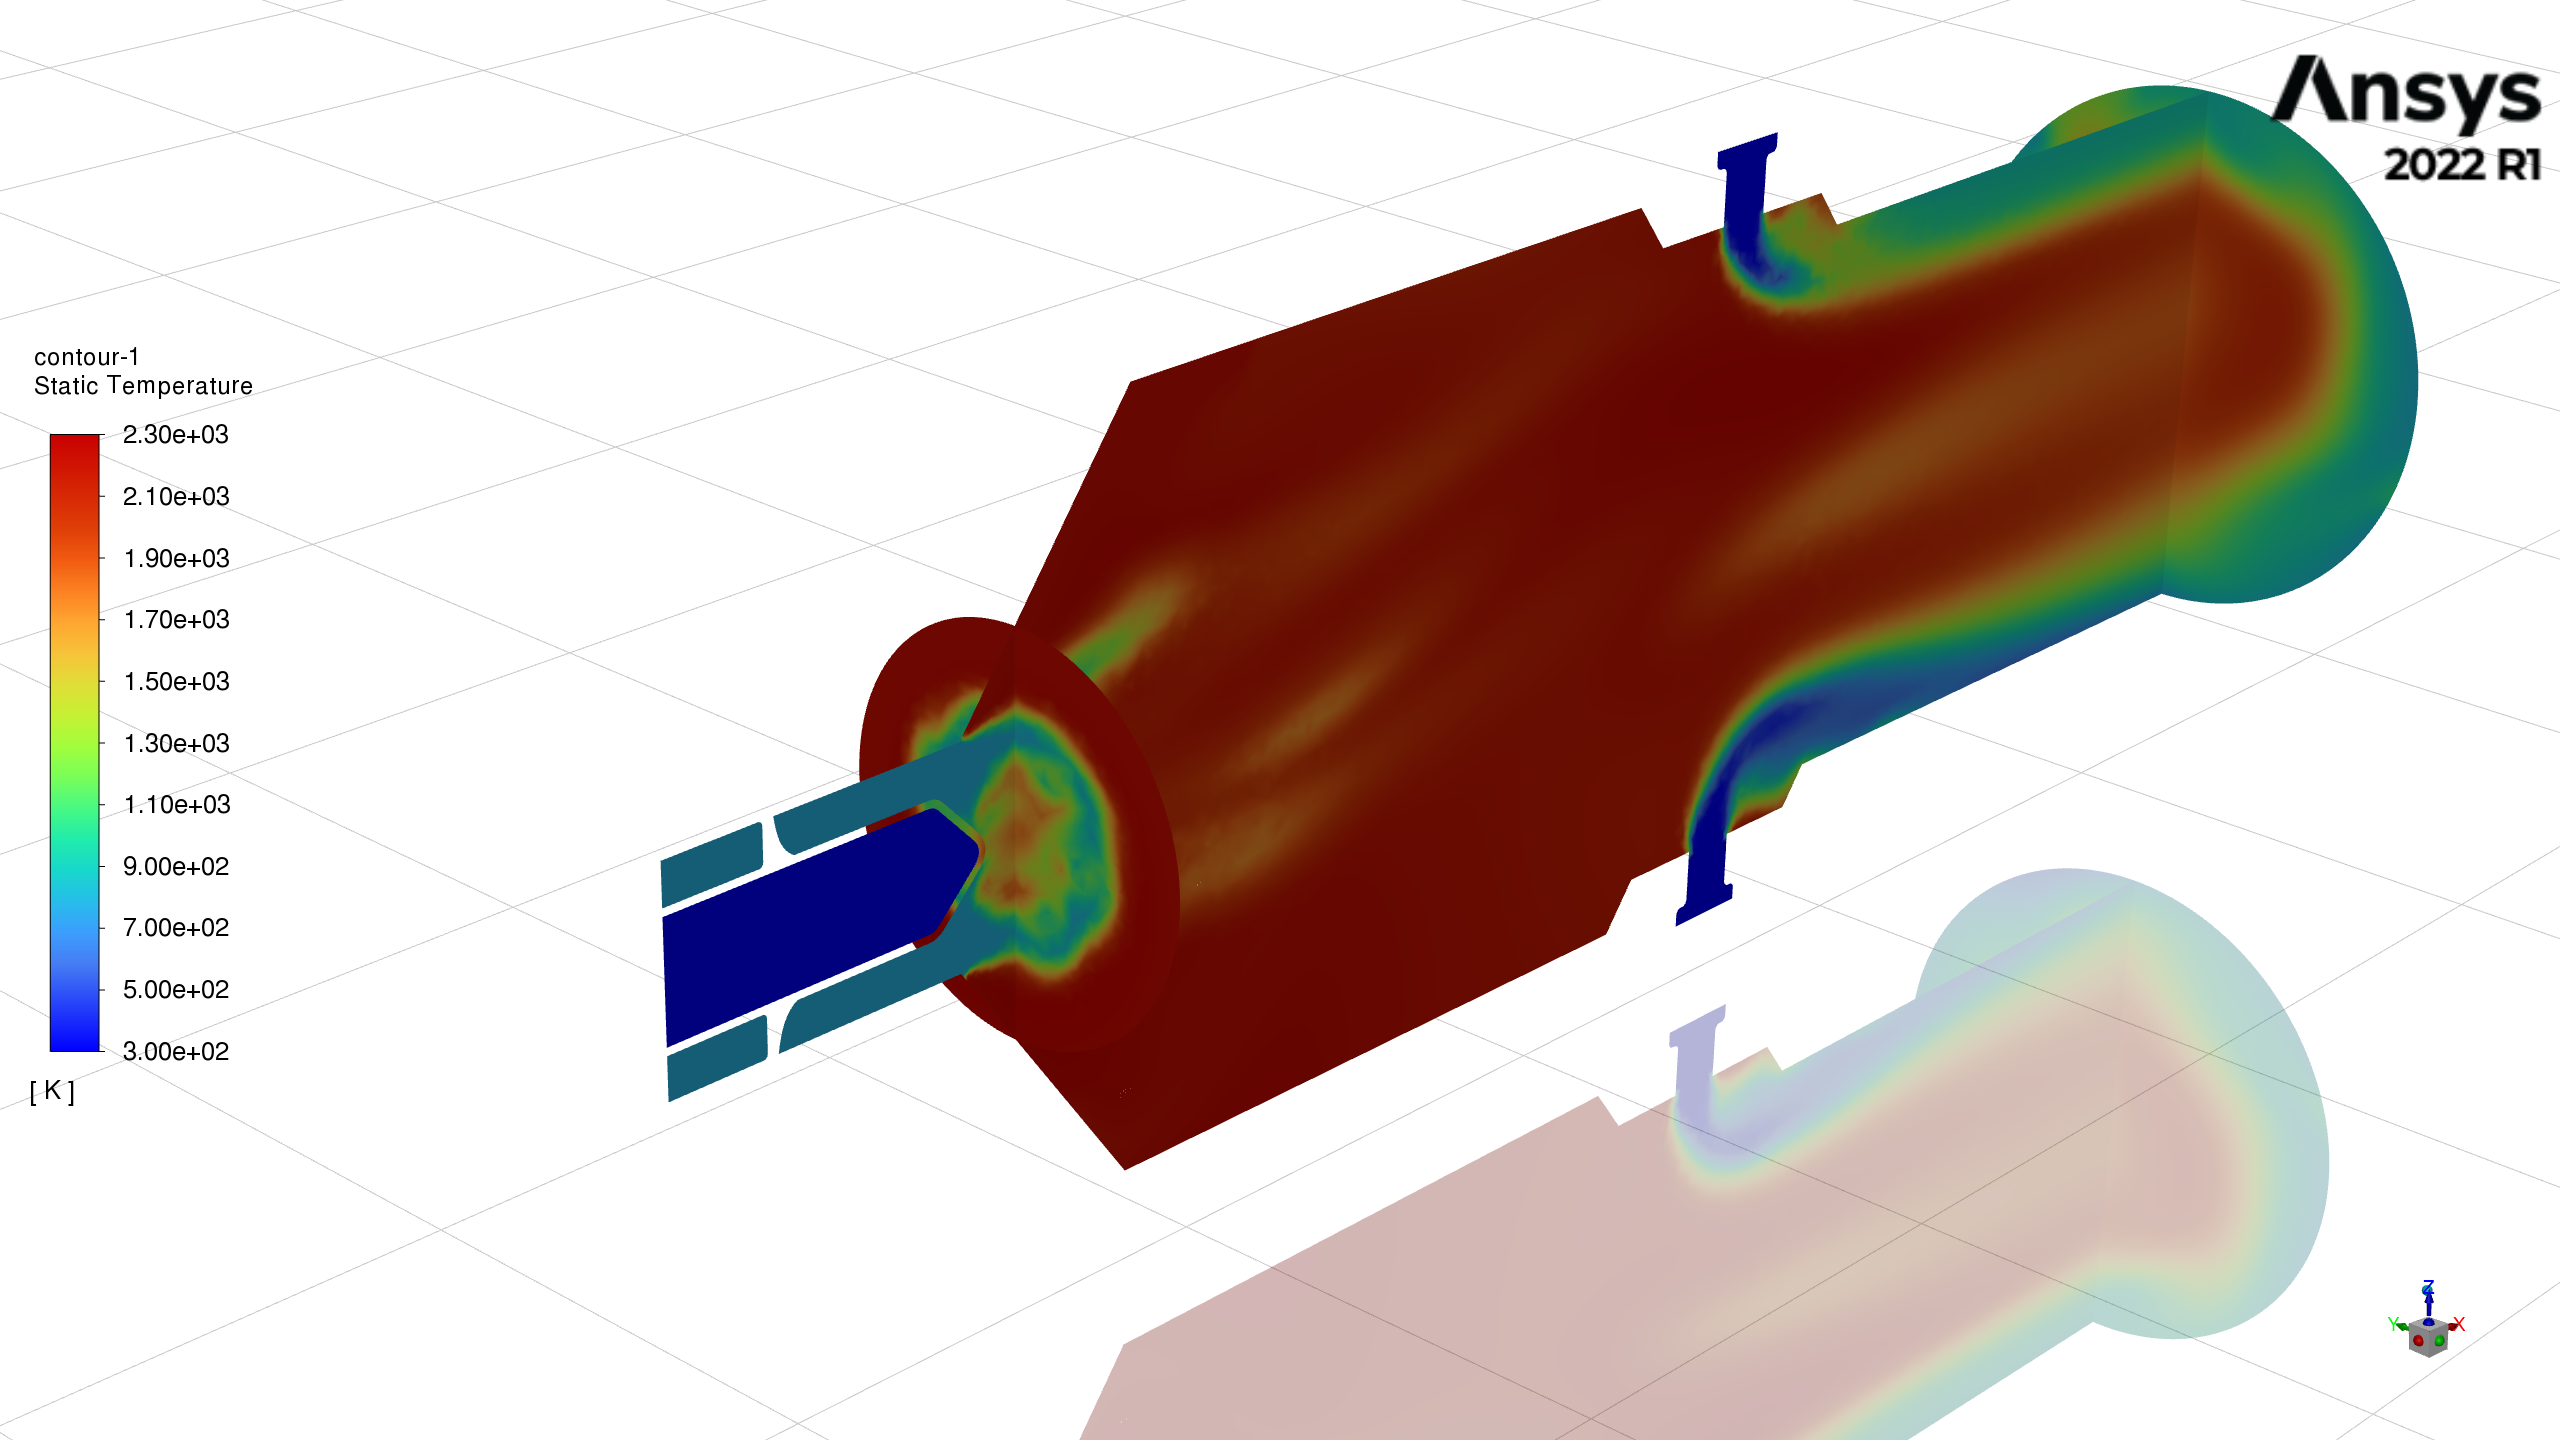
\includegraphics[width=\textwidth]{figs/pressure_front.png}
\end{subfigure}
\caption{Numerical mesh and setup.} \label{fig:numerical_setup}
\end{figure}


\autoref{fig:nh3species} shows the mass fraction of \ce{NH3}. It can be seen that in the fuel inlet, the mass fraction is 1. However, as soon as it mixes with the inlet air, the mass fraction reduces indicating that the NH3 is being consumed as the fuel. \autoref{fig:o2species} shows the mass fraction of \ce{O2}. Initially, it is the highest at the primary air inlet, and then starts being consumed as the oxidizer. However, a rise in the mass fraction can be seen when the secondary air is added.


The hydroxyl radical (\ce{OH}) is a key indicator of combustion activity and is commonly used to visualize flame fronts in reacting flows. Regions of high OH concentration correspond to zones where combustion is actively occurring, making it an effective marker for assessing flame stability and propagation characteristics. From \autoref{fig:ohspecies}, it can be observed that the flames being formed are not concentrated and are occupying the while combustor in the primary zone. This can be due to the fact the the fuel is present in excess allowing the flames to spread out.


Finally, we look at \ce{NOx} in \autoref{fig:nospecies}. It can clearly be seen that in the primary zone, the mass fraction of \ce{NO} is high. It is highly concentrated next to the flame front. However, after the secondary air is added, the mass fraction is reduced and is quite low near the outlet. 

\begin{figure}[H]
    \centering

    \begin{subfigure}[b]{0.49\textwidth}
        \centering
        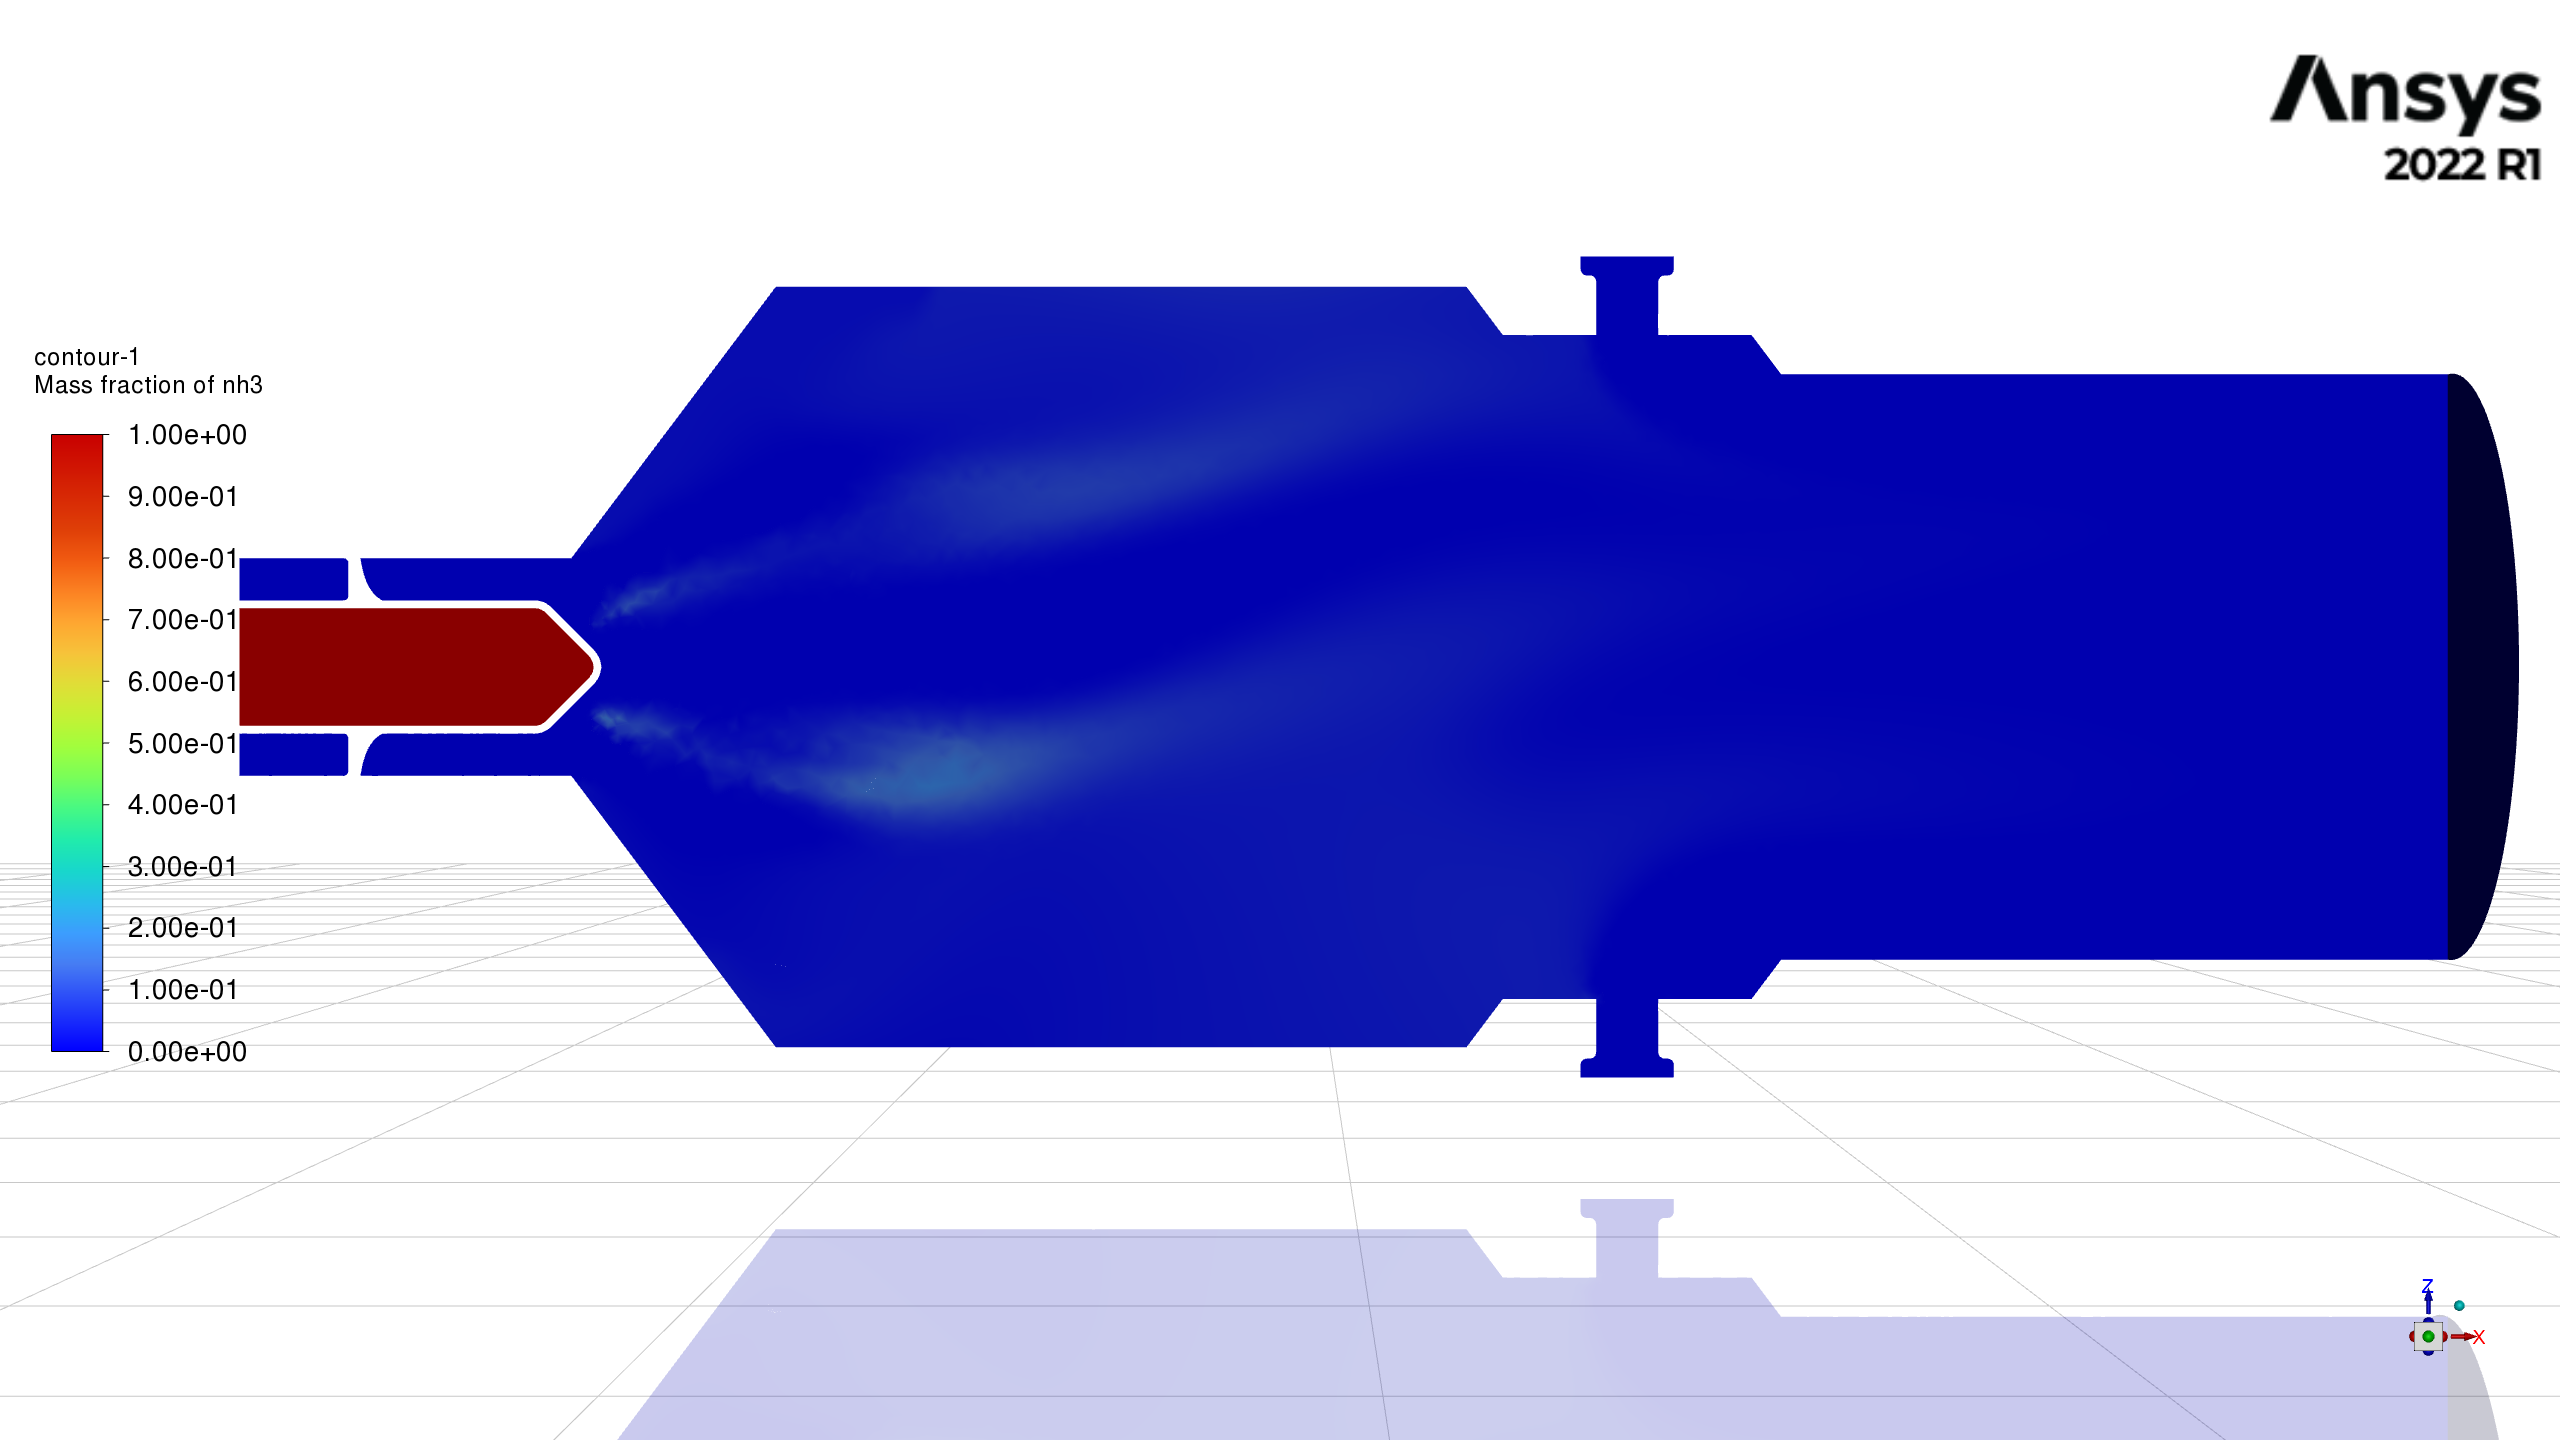
\includegraphics[width=\linewidth]{figs/species_nh3.png}
        \caption{Species \ce{NH3}}\label{fig:nh3species}
    \end{subfigure}
    \hfill
    \begin{subfigure}[b]{0.49\textwidth}
        \centering
        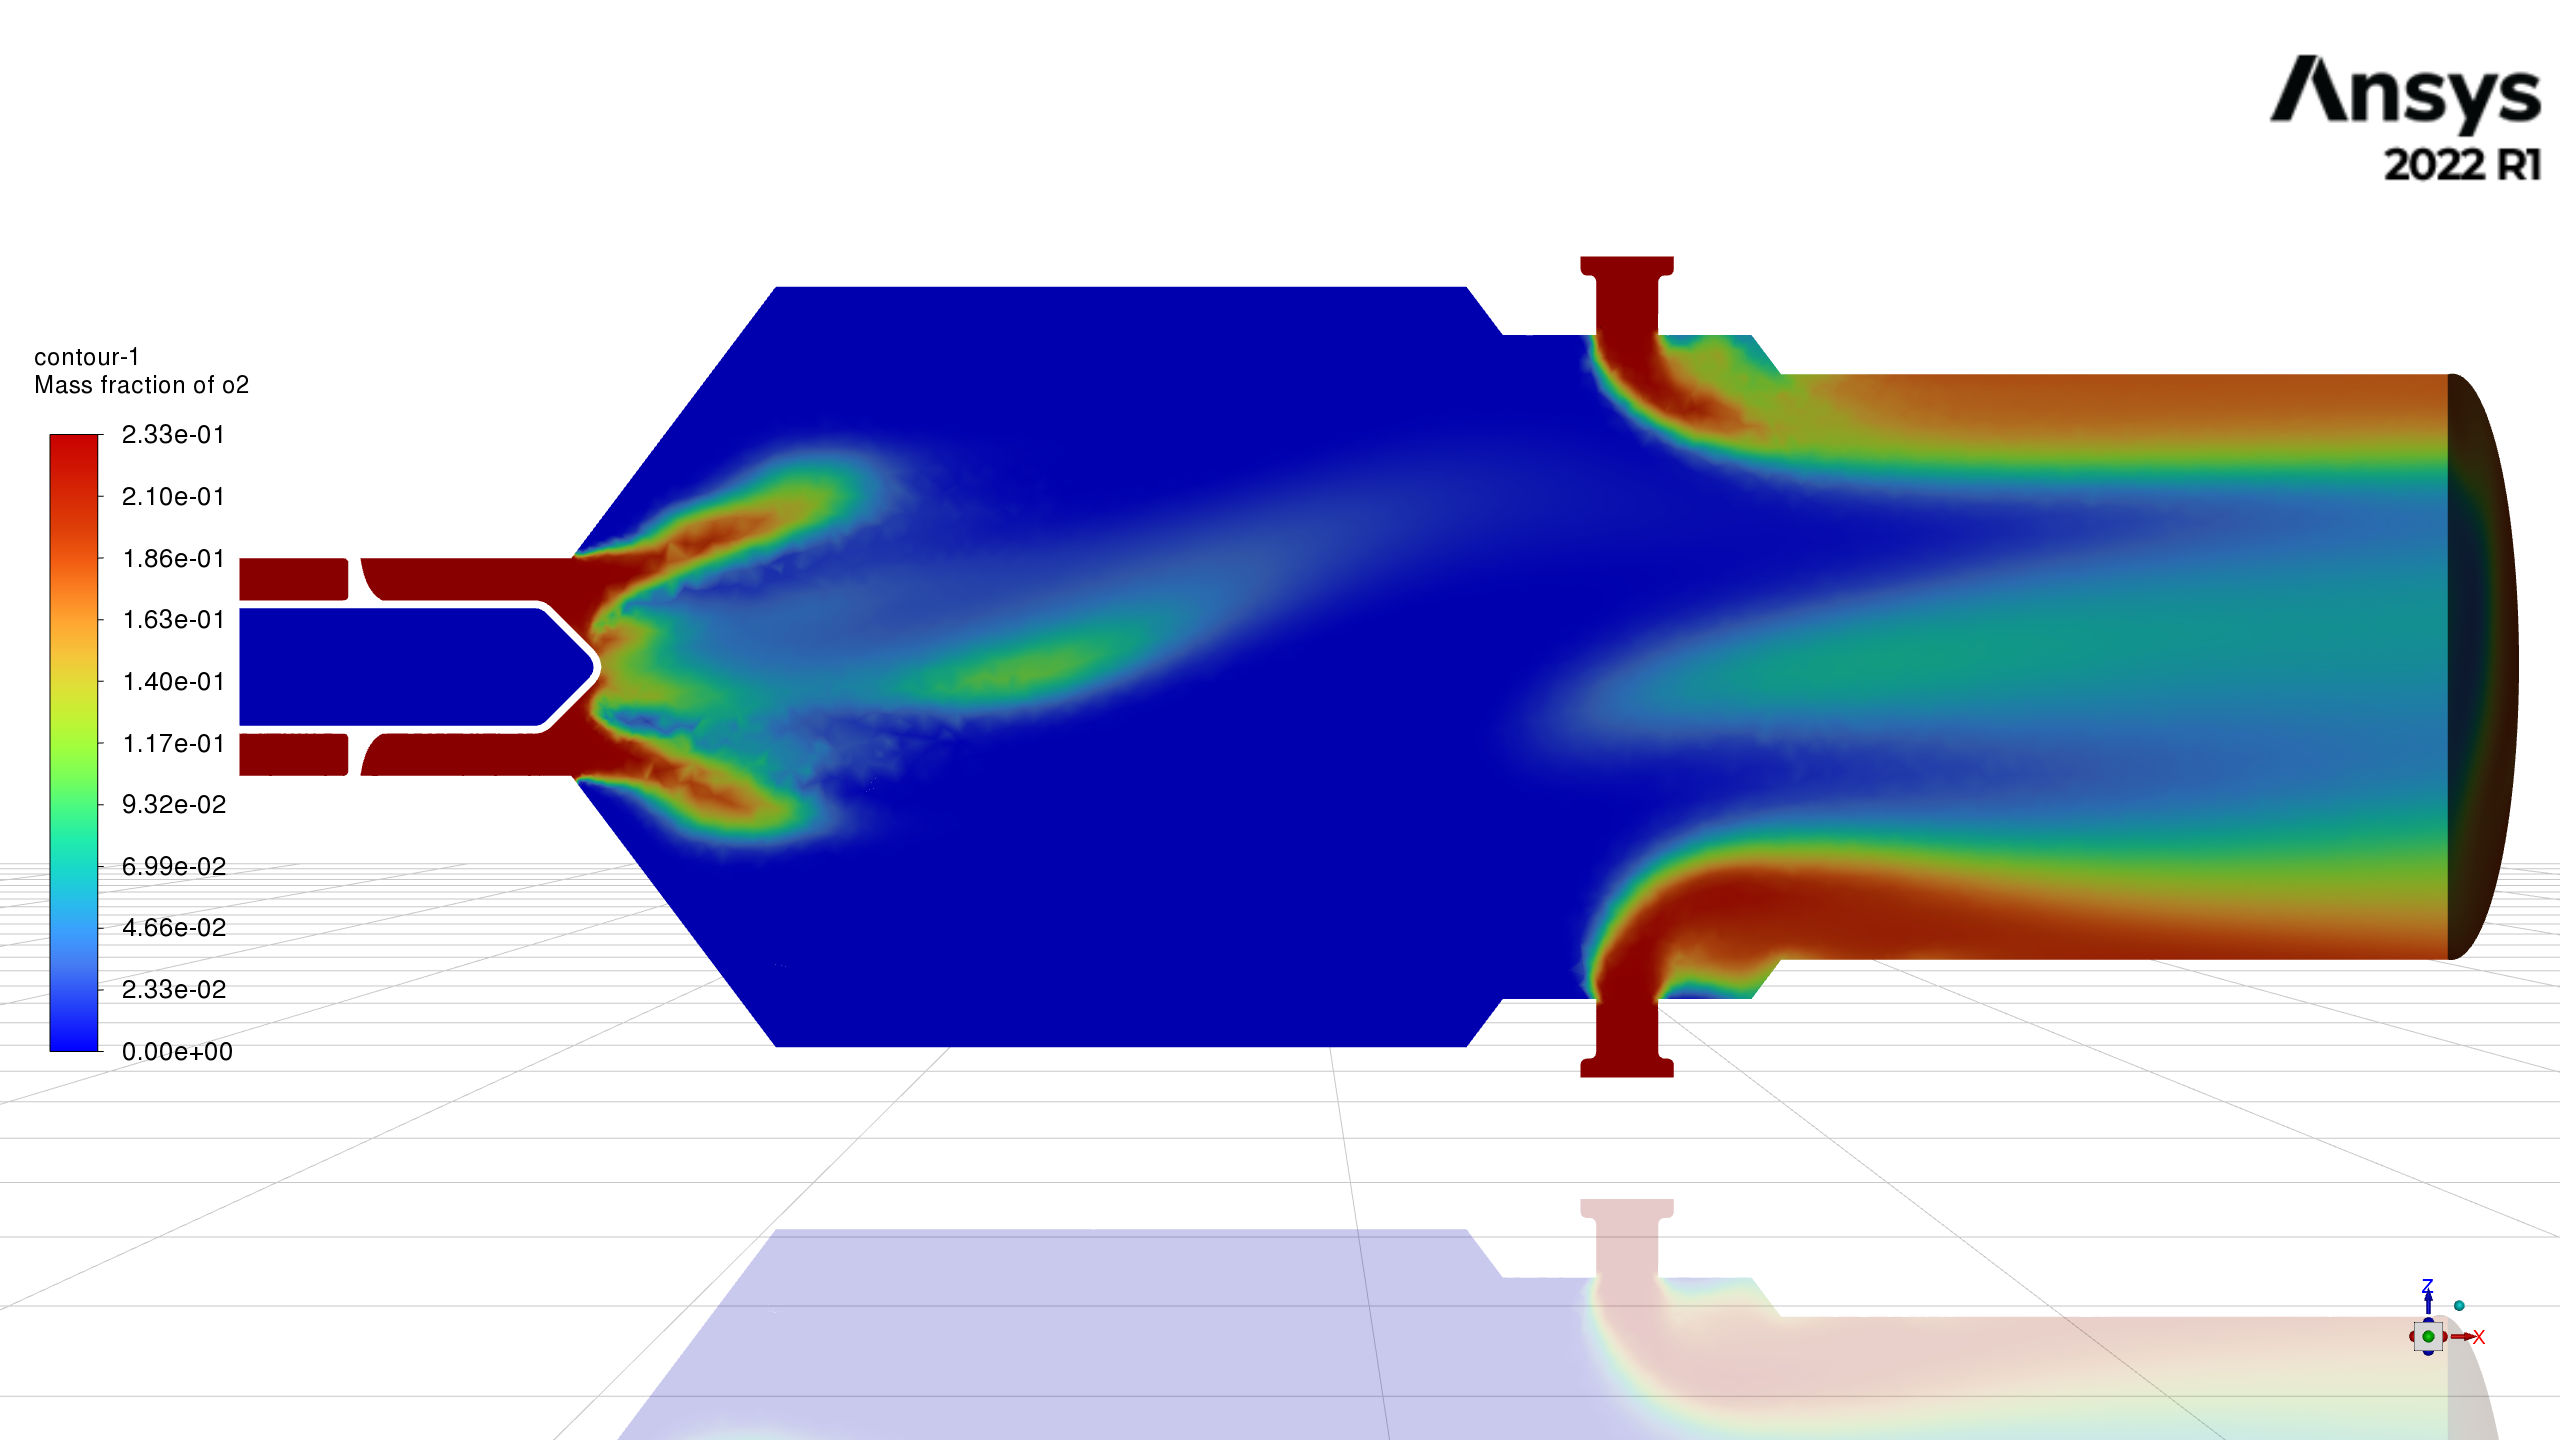
\includegraphics[width=\linewidth]{figs/species_o2.png}
        \caption{Species \ce{O2}}\label{fig:o2species}
    \end{subfigure}

    \vspace{0.5cm}

    \begin{subfigure}[b]{0.49\textwidth}
        \centering
        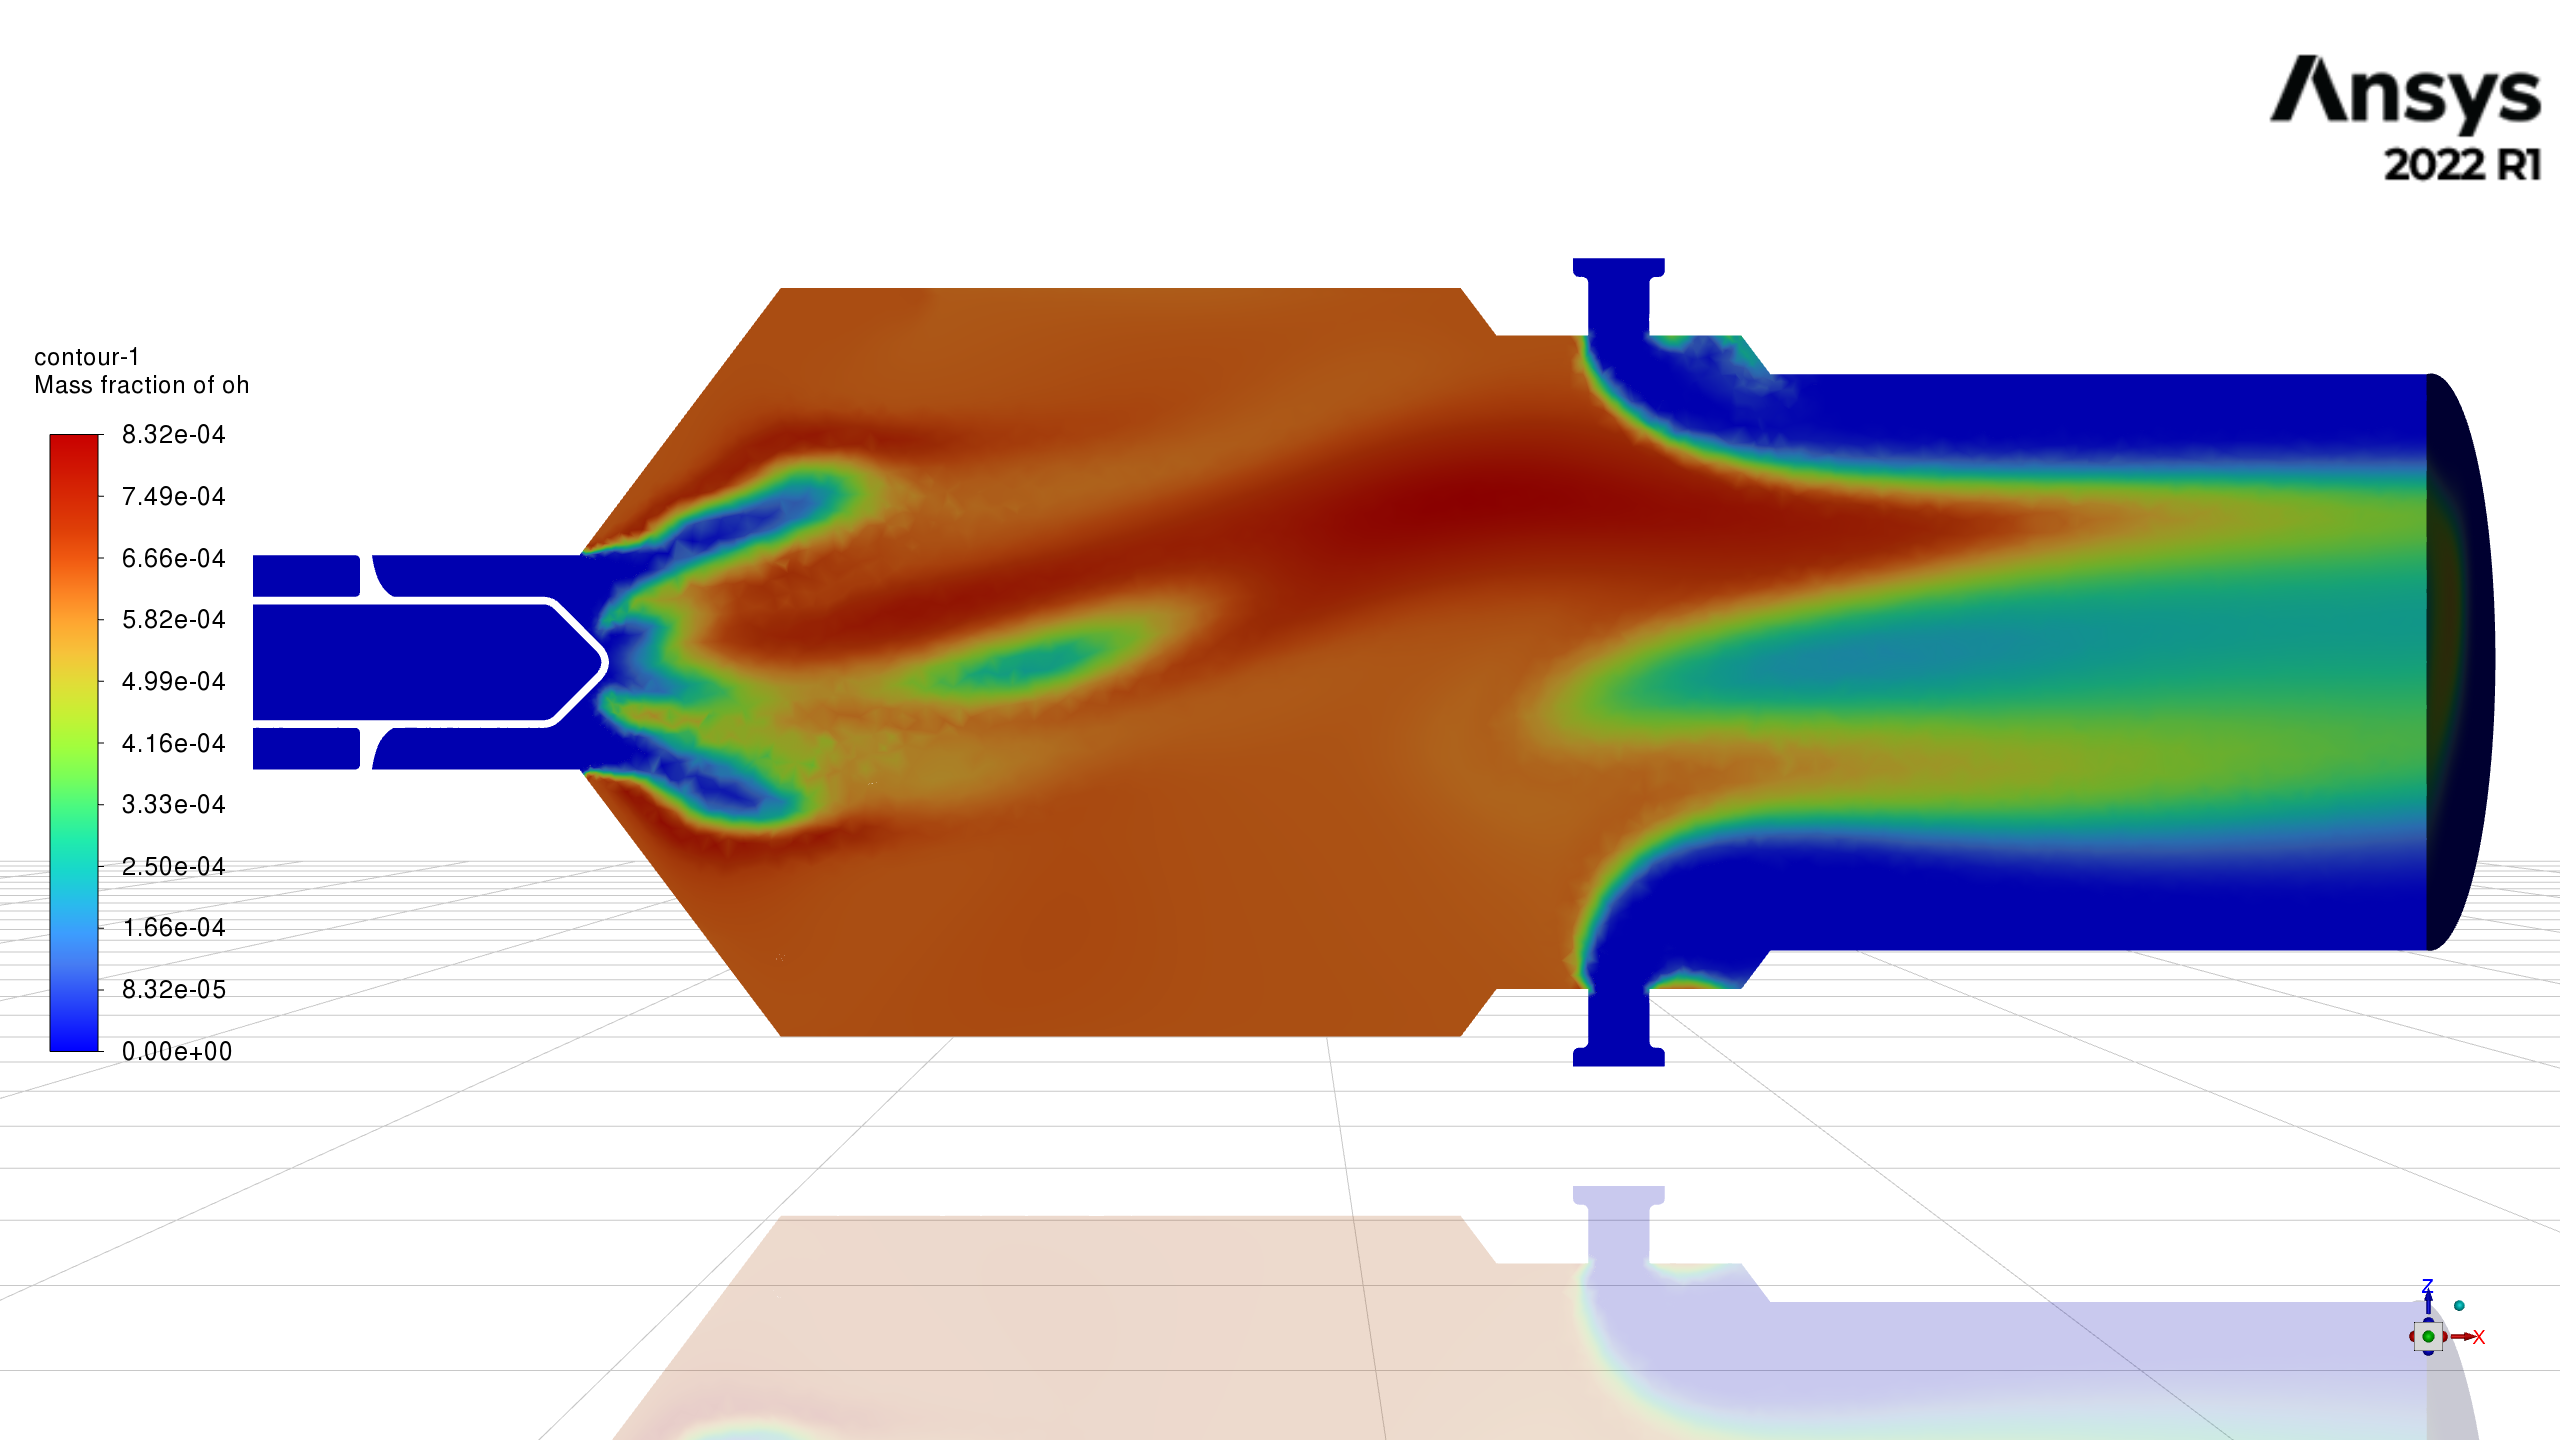
\includegraphics[width=\linewidth]{figs/species_oh.png}
        \caption{Species \ce{OH}}\label{fig:ohspecies}
    \end{subfigure}
    \hfill
    \begin{subfigure}[b]{0.49\textwidth}
        \centering
        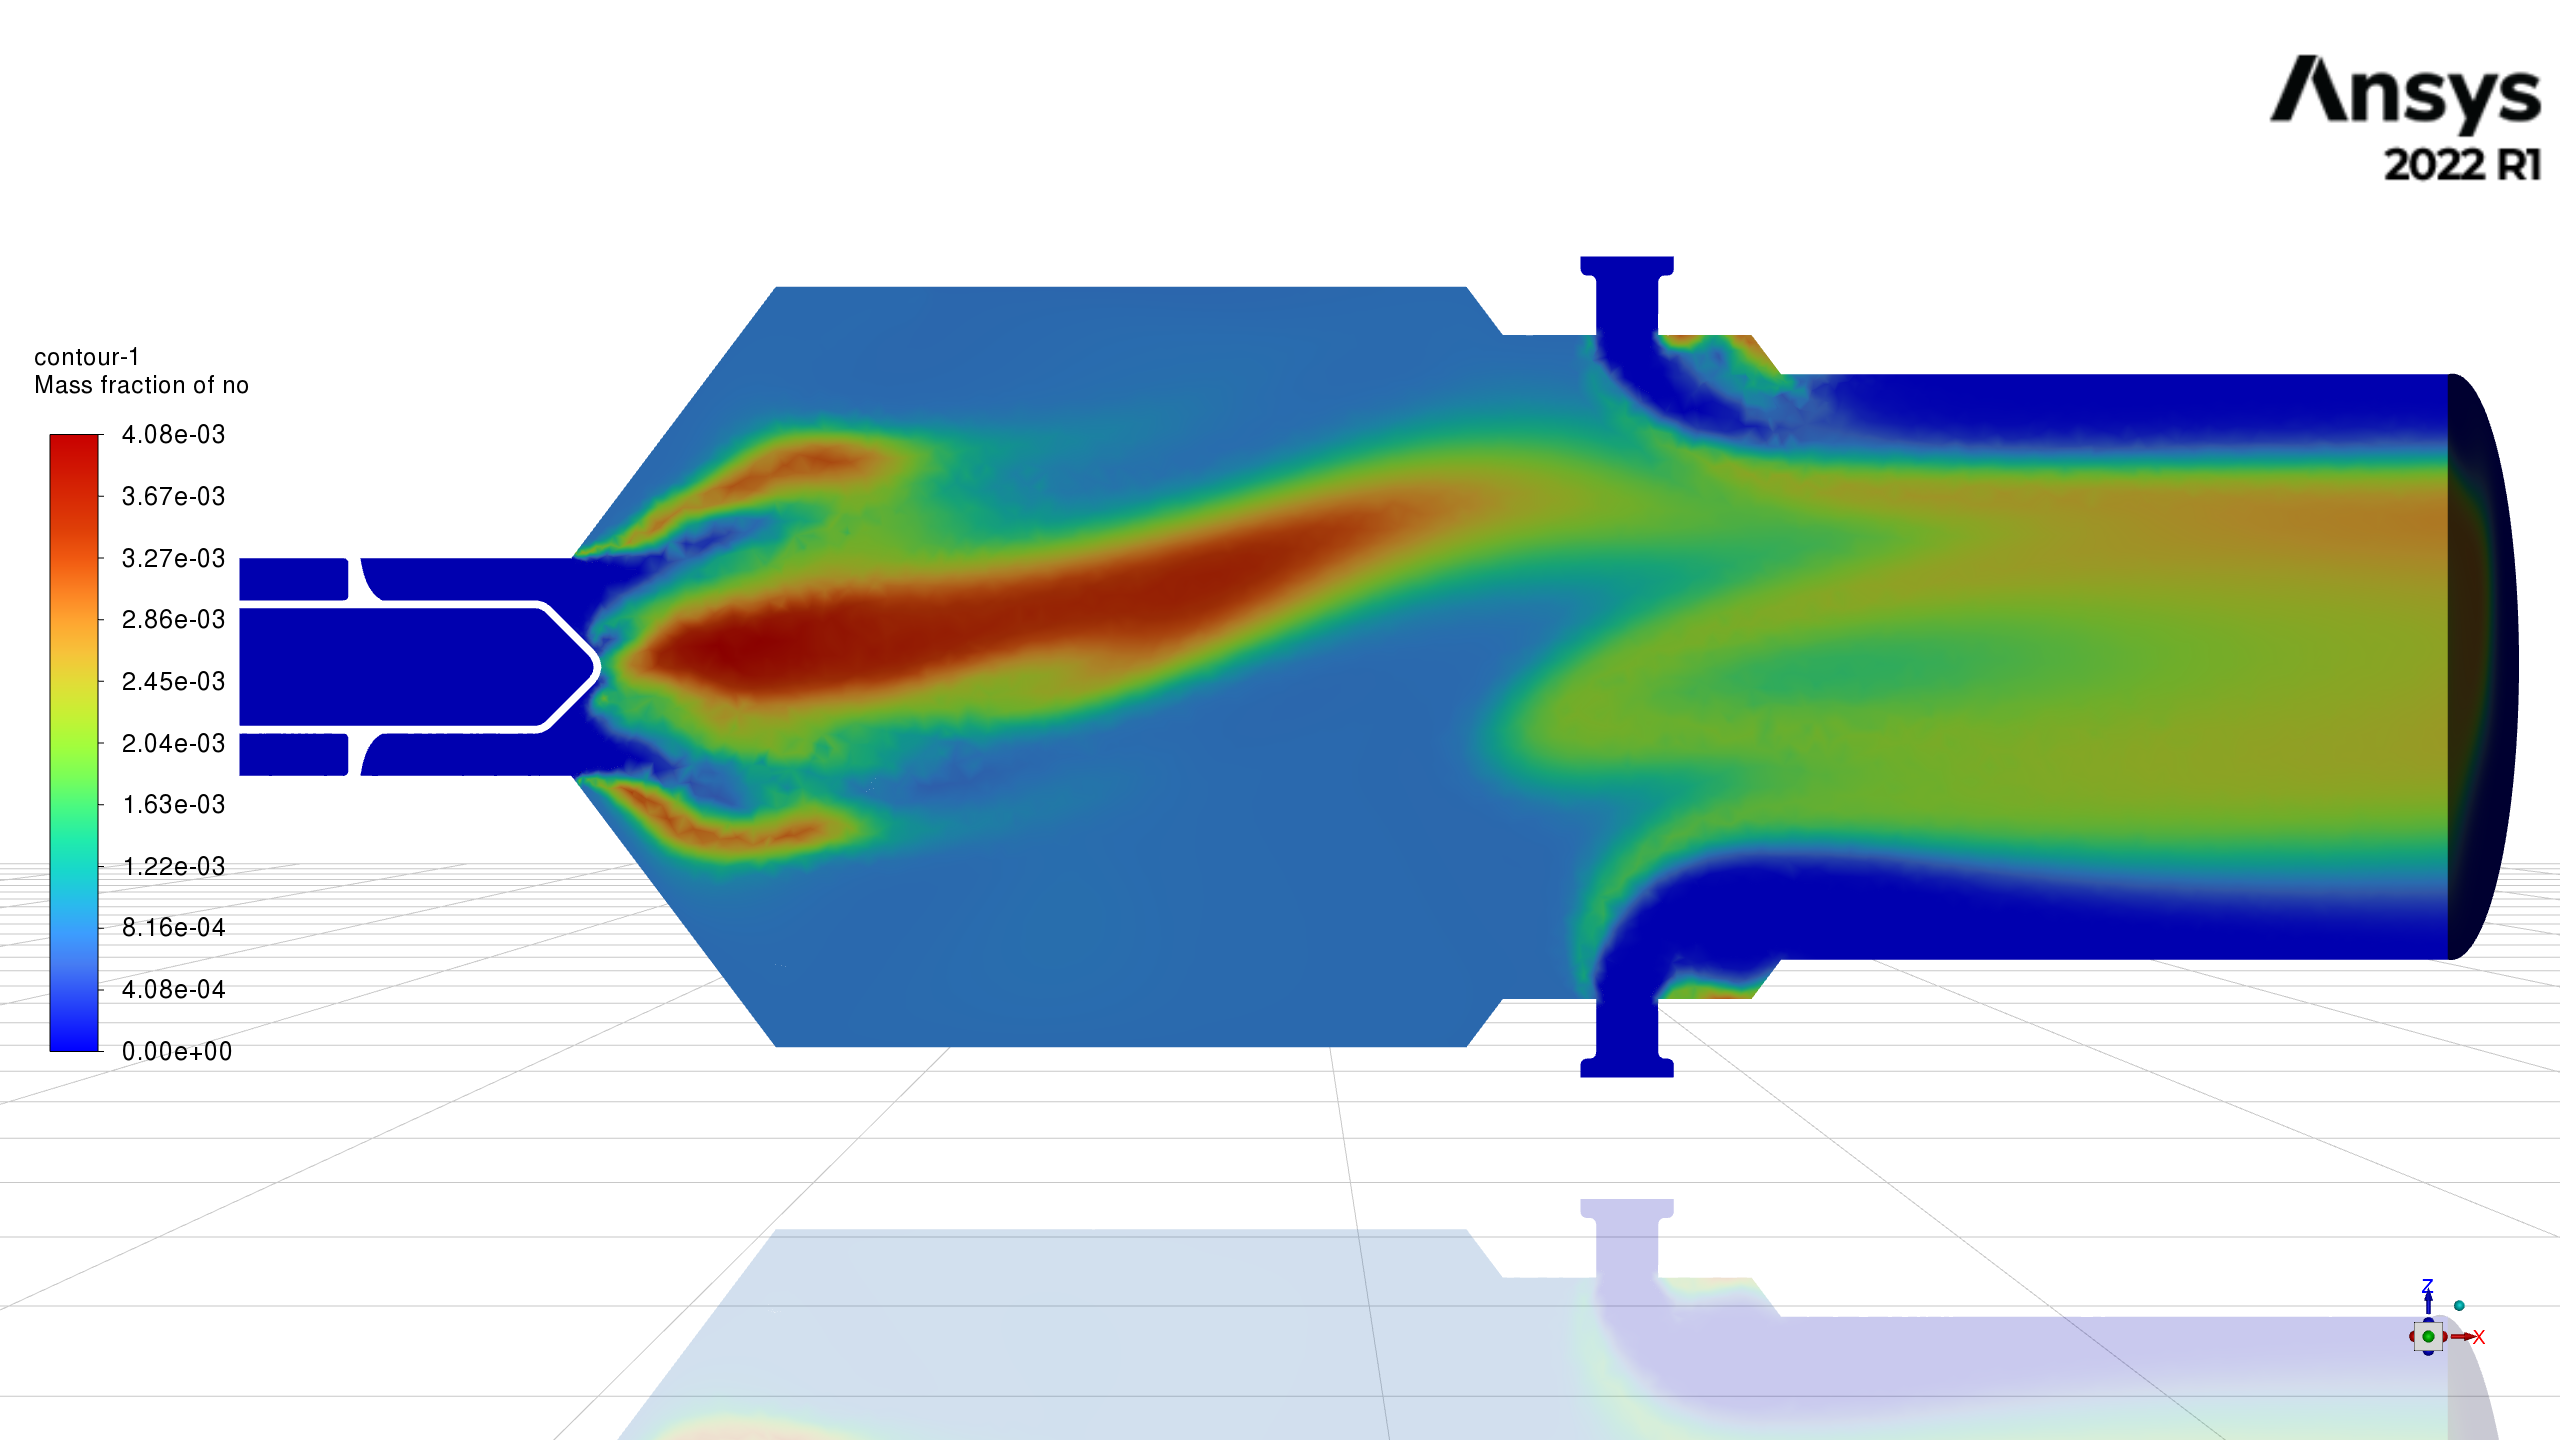
\includegraphics[width=\linewidth]{figs/species_no.png}
        \caption{Species \ce{NO}}\label{fig:nospecies}
    \end{subfigure}

    \caption{Mass fraction of various species across the combustor.}
    \label{fig:species_distro}
\end{figure}


\subsection{Discussion}

\autoref{tab:temp_comp} summarizes the temperatures obtained from cantera analysis as well as numerical analysis using ansys \footnote{Ansys results have been presented by visually looking at the contours presented in the previous subsection}. It can be seen that the temperatures obtained using ansys are higher than the ones computed using cantera. This can probably be due better modelling ability that comes with a 3D numerical simulation instead of simulating flames in 1D.

\begin{table}[H]
    \caption{Temperature comparison.}\label{tab:temp_comp}
    \label{tab:temp_comp}
    \centering
    \begin{tabular}{lll}
    \toprule
    \textbf{Zone} & \textbf{Cantera} & \textbf{ANSYS} \\ 
    \midrule
        Rich Zone & 2217.4 K &   2290 K \\
        Lean Zone & 1675.5 K &   1890 K \\
    \bottomrule
\end{tabular}
\end{table}

When looking at the emission results in \autoref{tab:nox_comp}, the results obtained by cantera are close to what has been seen in the literature in terms of \ce{NOx} production \cite{samuelsen2006rich}. However, the results from ansys show \ce{NOx} results much higher than expected. The reason cannot be determined at the moment.


\begin{table}[H]
    \caption{\ce{NOx} comparison.}\label{tab:nox_comp}
    \label{tab:temp_comp}
    \centering
    \begin{tabular}{lll}
    \toprule
    \textbf{Zone} & \textbf{Cantera} & \textbf{ANSYS} \\ 
    \midrule
    Combustor exit & 58.47 ppm &   2058 ppm \\
    \bottomrule
    \end{tabular}
\end{table}


\subsubsection{Known Errors}

Some know areas of errors are presented below:

\begin{itemize}
    \item Problems with combustion in the lean combustion zone: When performing the analysis using cantera, it was observed that no combustion was taking place in the lean burn zone even though a plug reactor was modelled in that region. The temperature does not change between the mixing zone and the outlet.
    
    \item Problems in the rich zone: At the exit of the rich zone, when looking the mass fraction of all the species, \ce{NH3} was being totally consumed even though the primary zone is supposed to have an equivalence ratio greate that 1. The cause of this problem is unknown and could be the cause of the problem discussed in the previous point.

    \item Limited CFD resources: CFD of reacting flow is time consuming. Therefore, the number of iterations that could be performed for testing and producing the results were limited. There results presented in this report were ran to 500 iterations only. Additionally, no mesh convergence study could be performed due to the same reason. This could have led to the false \ce{NOx} being reported by ansys simulations.
\end{itemize}